\documentclass[tikz,border=2pt]{standalone}
\usepackage{amsmath,amssymb}
\usepackage{pgfplots}
\usepgfplotslibrary{fillbetween}
\pgfplotsset{compat=1.18}

\begin{document}
% Y | X = x ~ Pois(x): conditional mean x and conditional variance x. The band mean +- one
% standard deviation widens with x, so Var(Y | X) = X is a function of X.
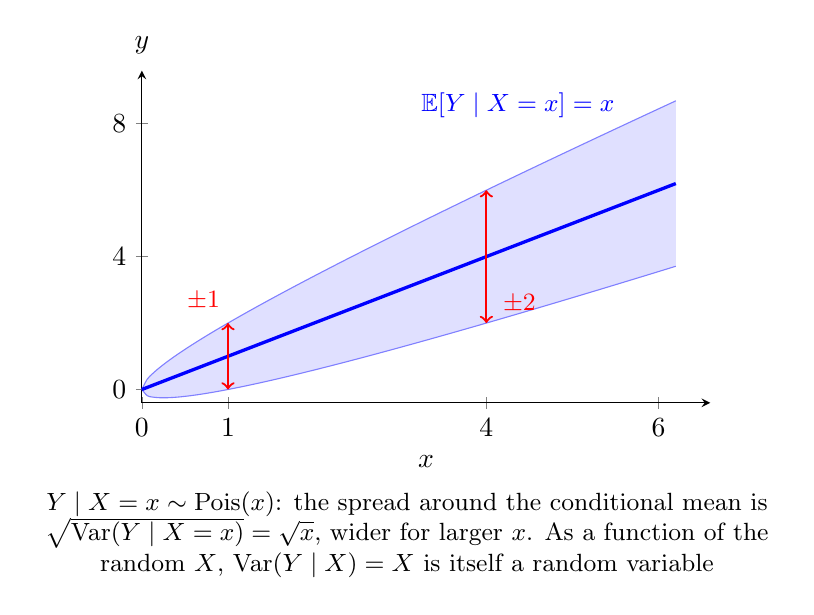
\begin{tikzpicture}
	\begin{axis}[
		axis lines=left, xmin=0, xmax=6.6, ymin=-0.4, ymax=9.6,
		xtick={0,1,4,6}, ytick={0,4,8},
		xlabel={$x$}, ylabel={$y$}, ylabel style={rotate=-90, anchor=south, at={(axis description cs:0,1.02)}},
		samples=100, smooth, width=8.8cm, height=5.8cm, clip=false
		]
		\addplot[name path=up, blue!50, domain=0:6.2] {x+sqrt(x)};
		\addplot[name path=down, blue!50, domain=0:6.2] {x-sqrt(x)};
		\addplot[blue!12] fill between[of=up and down];
		\addplot[blue, very thick, domain=0:6.2] {x};
		\draw[red, thick, <->] (axis cs:1,0) -- (axis cs:1,2);
		\draw[red, thick, <->] (axis cs:4,2) -- (axis cs:4,6);
		\node[red, anchor=south east, font=\small] at (axis cs:1.02,2.1) {$\pm1$};
		\node[red, anchor=west, font=\small] at (axis cs:4.08,2.6) {$\pm2$};
		\node[blue, anchor=south east, font=\small] at (axis cs:5.6,7.9) {$\mathbb{E}[Y\mid X=x]=x$};
	\end{axis}
	\node[anchor=north, font=\small, align=flush center, text width=9.4cm] at ([yshift=-2pt]current axis.outer south) {$Y\mid X=x\sim\operatorname{Pois}(x)$: the spread around the conditional mean is $\sqrt{\operatorname{Var}(Y\mid X=x)}=\sqrt x$, wider for larger $x$. As a function of the random $X$, $\operatorname{Var}(Y\mid X)=X$ is itself a random variable};
\end{tikzpicture}
\end{document}
